\chapter{Evaluation}
\label{chap:evaluation}


\section{Challenges}
\label{sec:challenges}

\subsection{CRF-dependent Distribution of Q-Values}
\label{subsec:crfdependentdistributionofQvalues}

The implementation of \cite{ng_cvpr07} has issues, which we were not able to solve. The problems show up first, when examining our created $Q$-$R$ histograms. The failure could be detected by computing these histograms for several images with known ground-truth CRFs. The distribution of the $Q$-values did not shift as predicted in theory. How these observations were obtained is described in the following.

Both, real-world and synthetic images were examined, and similar results were obtained. The real-world data was obtained by extracting linear RAW images from a camera and then manually applying a gamma function with different parameters $\gamma \in \left\{ 0.2, 0.4, 0.6, 0.8 \right\}$. For synthetic images, many -- about 1500 -- randomly sized filled circles with a random intensity each are put into an empty image. This image is then scaled up using bilinear interpolation to make the edges less sharp. As with real-world images, gamma curves were applied afterwards to mimic the camera response of a usual digital camera.

In theory, for $Q(R)$ histograms of images with mainly uniform distributed irradiance values,
\begin{enumerate}
	\item the mean intensity value $R_\text{mean}$ over all points in $S_\text{LISO}$ increases with decreasing $\gamma$. The reason is, that for instance for $\gamma = 0.2$, for small $R$ (low intensity values), the gamma curve $R = f(r) = r^{0.2}$ has a much larger slope than curves with larger $\gamma$. Remember, that $r \in [0; 1]$. Consequently, $R_\text{mean}$ increases. The second expected observation is, that
	\item $Q_\text{mean}$, similarly defined as $R_\text{mean}$, is smaller for small $\gamma$ than for large $\gamma$, because $Q(R)$ is directly related to the gamma curve parameter $\gamma$ (see \autoref{subsec:geoinvtheory}).
\end{enumerate}

The effects of the first assumption could be observed in all of our tests. Let $\gamma_1 < \gamma_2$. Then the distribution of $Q(R)$-values for histograms computed over images with $\gamma_1$ significantly shifts horizontally to the right (larger intensity values) in contrast to histograms computed over images with $\gamma_2$. Four example histograms for real-world images are presented in \autoref{fig:gamma_hists}.

\begin{figure}[tb]
	\centering
		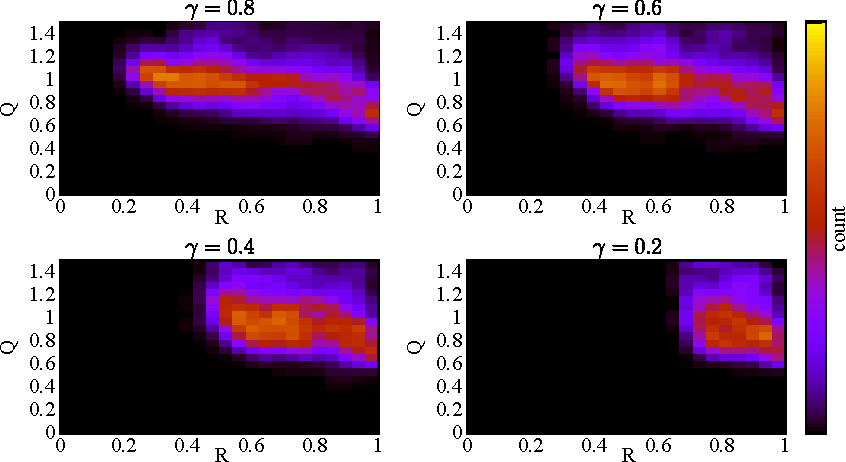
\includegraphics[width=0.95\textwidth]{histograms/geoinv_QR-diagramme.pdf}
	\caption[$Q$-$R$ histograms computed over images for different $\gamma$ curves]{$Q$-$R$ histograms computed over linear images, on which different gamma curves were applied. The upper left histogram shows the distribution of $Q(R)$-values for the largest value of $\gamma$. In the lower right, the $\gamma$-value is very small. Dark colors mean a low amount of occurring $Q(R)$-values in this area, while bright (yellow) colors stand for clusters corresponding to many $Q(R)$-values in $S_\text{LISO}$.}
	\label{fig:gamma_hists}
\end{figure}

But the second assumption turned out to be false for our implementation. The distribution of the $Q$-values does not shift vertically in the presented histograms, \hbox{i.e.} the $Q$-$R$ distribution does not align to the ground truth $\gamma$-line. The vertical distribution is very similar for all presented histograms, although $\gamma$ significantly differs.

Similar observations for both assumptions were obtained for all tested images. Hence, for instance for small values of $\gamma$, having almost no $Q$-values nearby the ground-truth, the subsequent optimization step fails consequently. The reason is, that it is heavily dependent on a reliable amount of properly detected points in $S_\text{LISO}$.



\clearpage

\subsection{Examination of Bayesian Inference}
\label{subsec:examinationofbayesianinf}

Another crucial part is the weighting of the points in $S_\text{LISO}$ as presented in \autoref{subsubsec:naivebayes}. Despite the problems with the $Q$-$R$-distribution described in \autoref{subsec:crfdependentdistributionofQvalues}, some of our obtained feature histograms appear quite similar to those presented in Ng's publication, but also significant mismatches were observed.

To create the feature histograms, we used a similar approach to the one in the previous section, gamma curves with $\gamma \in \left\{0.2, 0.4, 0.6\right\}$ were applied to both, synthetic and real-world images. Then the algorithm as presented in \autoref{subsec:geoinvalgo} is applied. Now we have $Q(R)$-histograms similar to those in \autoref{fig:gamma_hists}. These histograms represent the distribution of $Q(R)$-values over all points in $S_\text{LISO}$. Hence, this set of points is then classified into $S_\text{LPIP}$ and $S_\text{non-LPIP}$ by utilizing \autoref{eq:lpipclassification}. This procedure is repeated several times for different images and $\gamma$-values, resulting in two large sets of LPIPs and non-LPIPs, by concatenating all obtained $S_\text{LPIP}$ and $S_\text{non-LPIP}$. 

Due to the fact that the number of elements in $S_\text{LPIP}$ can significantly differ to $\left|S_\text{non-LPIP}\right|$, both sets are normalized to $[0; 1]$. This makes the histograms of $S_\text{LPIP}$ more comparable to the histograms of $S_\text{non-LPIP}$. The specific range of each feature is divided into a reliable number of bins and the normalized number of observations (points) per bin is stored. 

Our results are presented on page \pageref{fig:featurehistograms}. \autoref{fig:featurehistograms} shows the normalized histograms computed over more than 15 RAW images extracted from Hitachi HV-F22F. \autoref{fig:featurehistogramssynthetic} shows the normalized histograms of synthetic images.

The main differences to Ng's histograms are:
\begin{itemize}
	\item for small error values $E(R)$, our amplitude of non-LPIPs is significantly larger than Ng's. There, the histograms for the the two classes are even quite similar in contrast to those in \autoref{subfig:er} or \autoref{subfig:ersynthetic}.
	\item Also the second feature does not differ a lot for LPIPs and non-LPIPs in the paper, while our histograms are relatively dissimilar.
	\item The values of the third feature in \autoref{subfig:lambda} and \autoref{subfig:lambdasynthetic} range from negative to positive values, whereas in the paper, the values for this feature are all negative ($< 0$).
\end{itemize}

\begin{figure}[tbp]
  \centering
  \subfigure[Error function value $E(R)$]{
    \label{subfig:er}
    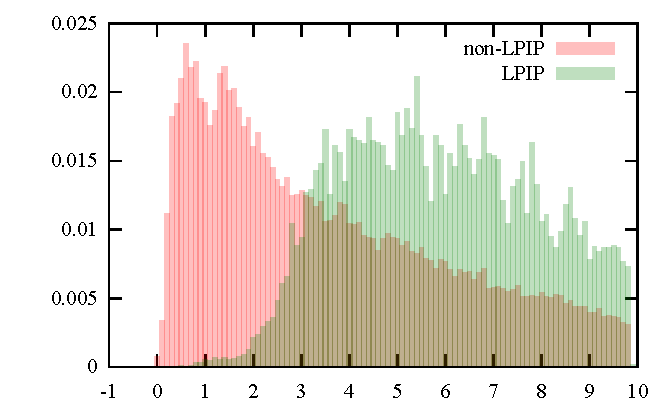
\includegraphics[width=0.31\textwidth]{plots/feature0.pdf} 
  }
  \subfigure[Gradient magnitude $\left|\mathrm{grad}(R)\right|$]{
    \label{subfig:gradientmagnitude}
    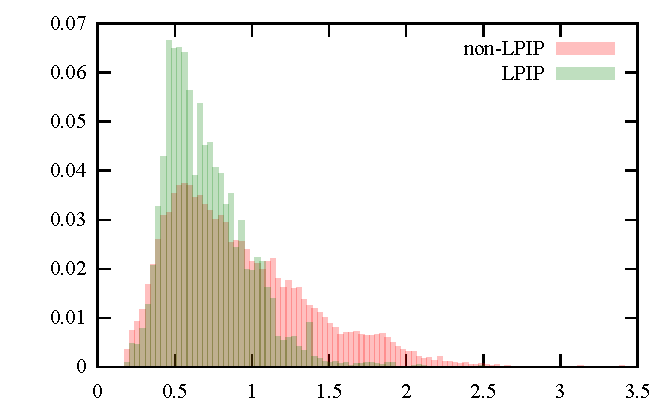
\includegraphics[width=0.31\textwidth]{plots/feature1.pdf} 
  }
  \subfigure[Lambda $\lambda$]{
    \label{subfig:lambda}
    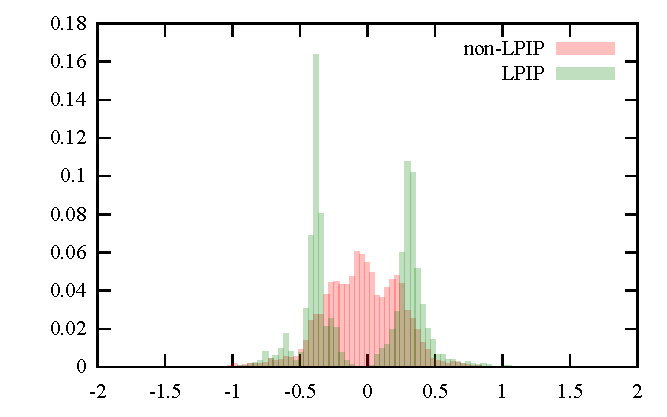
\includegraphics[width=0.31\textwidth]{plots/feature2.pdf} 
  }
  \subfigure[Total mass $m_0$]{
    \label{subfig:totalmass}
    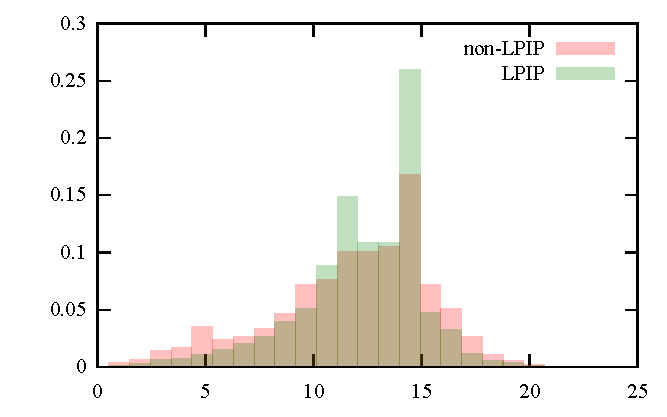
\includegraphics[width=0.31\textwidth]{plots/feature3.pdf} 
  }
  \subfigure[Centroid $m_1$]{
    \label{subfig:centroid}
    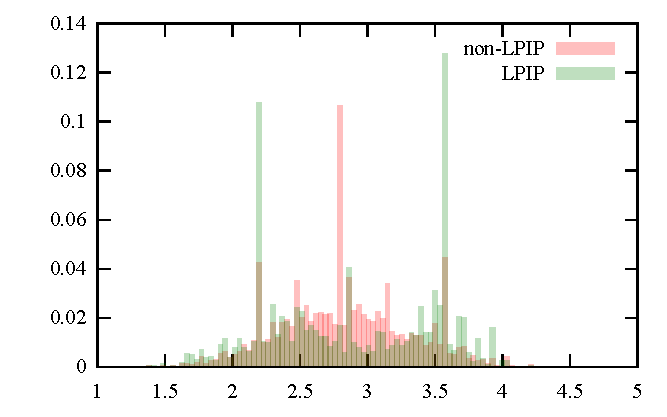
\includegraphics[width=0.31\textwidth]{plots/feature4.pdf} 
  }
  \subfigure[Radius of Gyration $m_2$]{
    \label{subfig:gyration}
    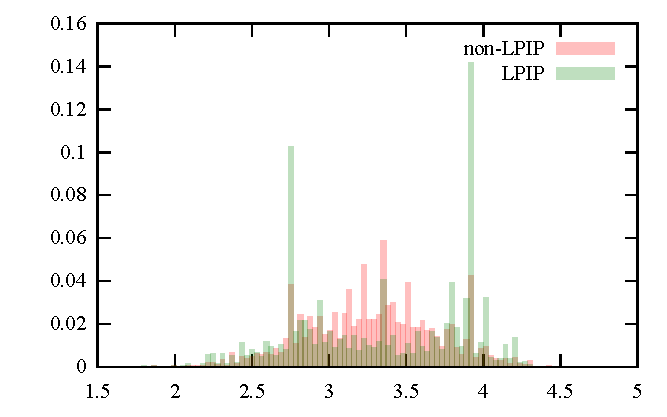
\includegraphics[width=0.31\textwidth]{plots/feature5.pdf} 
  }
  \caption{Normalized feature histograms generated with \emph{RAW} images}
  \label{fig:featurehistograms}
\end{figure}

\begin{figure}[tbp]
  \centering
  \subfigure[Error function value $E(R)$]{
    \label{subfig:ersynthetic}
    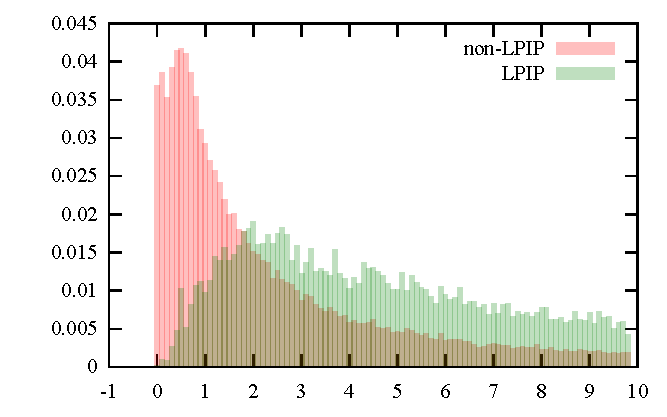
\includegraphics[width=0.3\textwidth]{plots/featureSynth0.pdf} 
  }
  \subfigure[Gradient magnitude $\left|\mathrm{grad}(R)\right|$]{
    \label{subfig:gradientmagnitudesynthetic}
    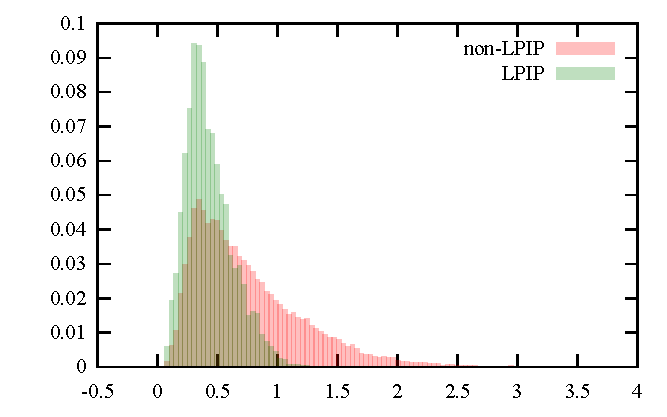
\includegraphics[width=0.3\textwidth]{plots/featureSynth1.pdf} 
  }
  \subfigure[Lambda $\lambda$]{
    \label{subfig:lambdasynthetic}
    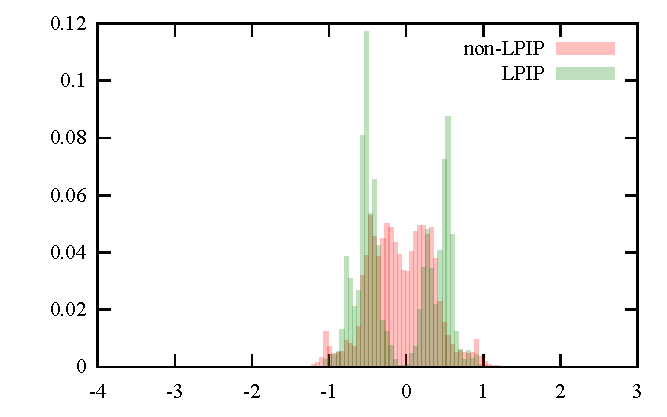
\includegraphics[width=0.3\textwidth]{plots/featureSynth2.pdf} 
  }
  \subfigure[Total mass $m_0$]{
    \label{subfig:totalmasssynthetic}
    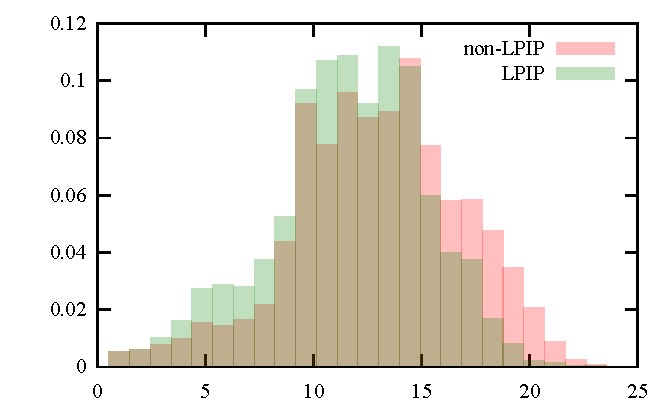
\includegraphics[width=0.3\textwidth]{plots/featureSynth3.pdf} 
  }
  \subfigure[Centroid $m_1$]{
    \label{subfig:centroidsynthetic}
    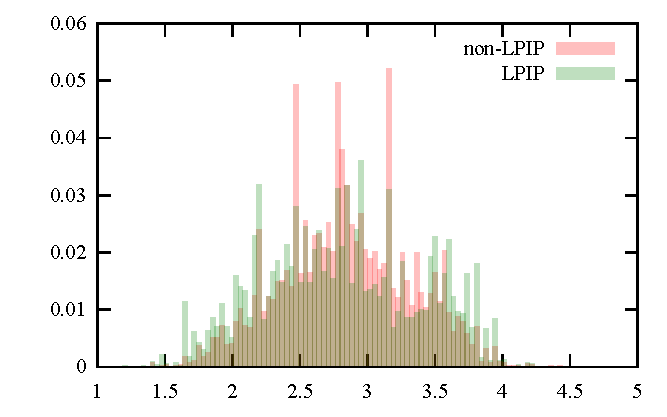
\includegraphics[width=0.3\textwidth]{plots/featureSynth4.pdf} 
  }
  \subfigure[Radius of Gyration $m_2$]{
    \label{subfig:gyrationsynthetic}
    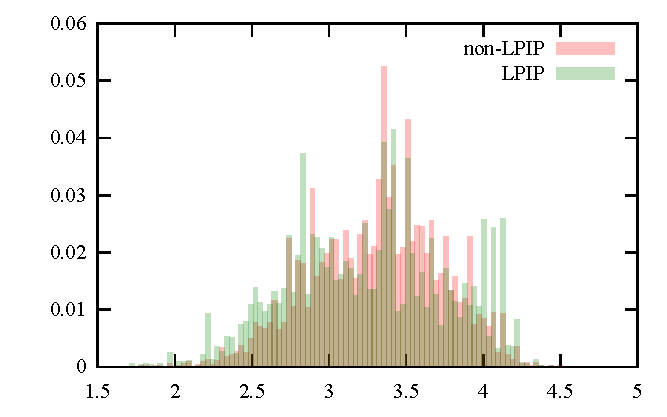
\includegraphics[width=0.3\textwidth]{plots/featureSynth5.pdf} 
  }
  \caption{Normalized feature histograms generated with \emph{synthetic} images}
  \label{fig:featurehistogramssynthetic}
\end{figure}




\clearpage

\subsection{Problem-solving Approach}
\label{subsec:problemsolving}

The main problem is described in \autoref{subsec:examinationofbayesianinf}, our implementation fails finding a reliable amount of points around the ground-truth line in $Q$-$R$ space. Consequently, the feature histograms used for the classification can not be correct. An approach for further efforts in localizing the actual error source, either a missing implementation detail or something being wrong with the theory part, is presented in the following.

For this approach, the value of the error function is ignored, \hbox{i.e.} every point is taken into $S_\text{LISO}$. Hence, all points of the image are classified into $S_\text{LPIP}$ and $S_\text{non-LPIP}$ (analogous to \autoref{eq:lpipclassification}). This is applied three times to a particular image, using three different gamma curves, where $\gamma \in \left\{0.2, 0.4, 0.6\right\}$. 

Next, the three distinct ``LPIP-maps'' (containing only the classified LPIPs at their specific position from the original image) $L_{0.2}$, $L_{0.4}$ and $L_{0.6}$ are extracted and combined afterwards. $L_{\gamma}$ denotes the LPIP-map for the particular $\gamma$. The combination is done by first creating an empty RGB image and second using the three LPIP-maps as the three channels, where $L_{0.2}$ is used as the red, $L_{0.4}$ as the green and $L_{0.6}$ as the blue channel. 

With this image, points, which are classified as LPIPs for all three gamma curves, can be extracted easily, because they appear white. In the example from \autoref{fig:LPIPmaps}, about $14 \%$ of all colored pixels fulfill this condition. Now, these points can be analyzed to get further insight.

\vspace{0.7cm}

\begin{figure}[htbp]
  \centering
  \subfigure[original image]{
    \label{subfig:original image}
    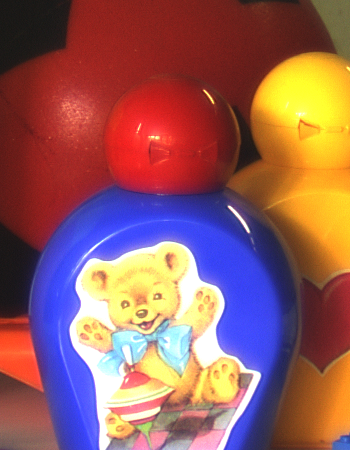
\includegraphics[width=0.315\textwidth]{liso_maps/small.png} 
  }
  \subfigure[combined LPIP-map]{
    \label{subfig:combined LPIP-map}
    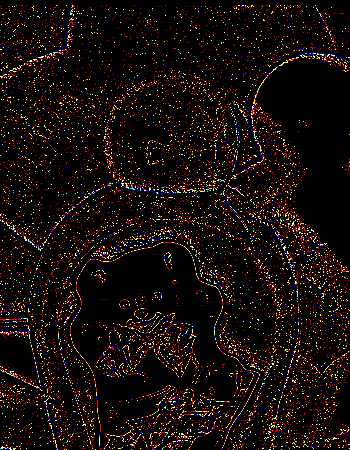
\includegraphics[width=0.315\textwidth]{liso_maps/all.png} 
  }
  \subfigure[intersection of LPIP-maps]{
    \label{subfig:white points}
    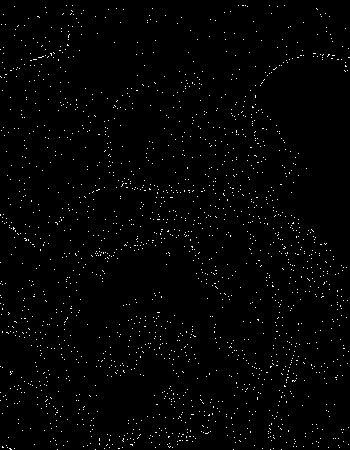
\includegraphics[width=0.315\textwidth]{liso_maps/white_only.png} 
  }
  \caption[Original image and combined LPIP-map]{Original image, combined LPIP-map and intersection of all channels (white pixels).}
  \label{fig:LPIPmaps}
\end{figure}



\clearpage

\section{Capabilities of Data Acquisition}
\label{sec:capabilitiesofdataacqu}

In this and the next two evaluation appraoches, only the method by Lin et al. is examined. It requires a sufficienctly large, representative set of edge samples. If not enough data could be gathered before, the optimization step can not produce any good results. Hence, the data acquisition step, taking place before the actual CRF estimation algorithm, is analyzed.


\subsection{Crucial Parameters}
\label{subsec:parameterIntroduction}

Tests have shown that the amount of accepted patches and thus the size of the observation set is heavily dependent on the settings of two parameters:
\begin{enumerate}
	\item $\epsilon_\text{min}$, threshold for the minimum distance between the two region colors $C_1$ and $C_2$ and
	\item $\epsilon_\text{max}$, threshold for the maximum distance of the colors within a region $C_1$ or $C_2$.
\end{enumerate}
For all distance computations the common Euclidean norm is used, although other distance metrics are possible.

At first, the boundaries $B$ for both parameters have to be found, what is straightforward due to the use of normalized RGB colors and the Euclidean norm. All points in the three-dimensional normalized RGB space lie in a cube spanned by the unit vectors $(1, 0, 0)^\mathrm{T}$, $(0, 1, 0)^\mathrm{T}$ and $(0, 0, 1)^\mathrm{T}$ with its origin at $(0, 0, 0)^\mathrm{T}$, where $\vec{x}^\mathrm{T}$ denotes the transposed vector $\vec{x}$. Hence, the largest distance inside that cube -- considering the Euclidean norm -- is $\sqrt{1^2+1^2+1^2} = \sqrt{3} \ \ \Rightarrow \  \epsilon_\text{min}, \epsilon_\text{max} \in B = [0; \sqrt{3}]$.

Knowledge about the impact of these parameters on the dataset quality is of high relevance for a reasonable evaluation. If $\epsilon_\text{min}$, the minimum distance between $C_1$ and $C_2$ -- \hbox{i.e.} a measurement for how dissimilar the colors have to be -- is too small, the line between the region colors can also be very short. That might not be a problem in theory, but in practice, due to the computation of the region colors (just taking the mean color of all colors within a region bounded by the size of the patch and the edge inside the patch), the variance of the colors inside the region highly affects the reliability of the following CRF estimation for a small $\epsilon_\text{min}$. This variance is covered by $\epsilon_\text{max}$, thresholding the maximum Euclidean distance of the colors within a region. This can be seen as the degree of similarity of the respective colors. Hence, the obvious choice for the two parameters considering optimal conditions (no noise and regions with uniform colors) would be $\epsilon_\text{min} \rightarrow \text{max}(B) = \sqrt{3};\ \ \epsilon_\text{max} = \text{min}(B) = 0$.

The expectation on the parameters is, that they have an opposing behavior. $\epsilon_\text{max}$ is related to the number of found patches, \hbox{i.e.} the larger the value of $\epsilon_\text{max}$ gets, the more patches will be found. Large values of $\epsilon_\text{min}$ on the other hand will result in a small number of patches. 

That all leads to the conclusion, that first $\epsilon_\text{min} > \epsilon_\text{max}$ and second the difference $\epsilon_\text{min} - \epsilon_\text{max}$ should be as large as possible. Third, a sufficiently large number of patches must be extracted.  


\subsection{Color Coverage Factor}
\label{subsec:colorCoverageFactor}

Not only the number patches is important, but also the coverage of the color space by the set of color triples. A large amount of collected data does not necessarily lead to a good CRF estimation. The reason is that the colors in the dataset (region colors and edge color) might be equal or very similar. This would result in the same corrupting effect on the final optimization step as having just a very small dataset -- an optimization with respect only to a sparse $R$ coverage. So another important variable arises: $\beta$, the \emph{coverage factor}, which measures the ratio of the coverage of all colors in the dataset (all colors for each patch $C_1$, $C_2$ and $C_{\text{edge}}$) over the occurring colors in the entire image. The computation is done by a clustering approach. Each dimension of the normalized RGB space is split into $N$ equidistant parts, where $N = 16$. As a result there is a total of $16^3$ clusters delimited by a three-dimensional lattice defined by the split points. All important steps for the computation of $\beta$ are presented in \autoref{alg:ccfc} on page \pageref{alg:ccfc}. Note that $\beta$ is not based on the entire RGB space, but on the parts of it which are used by the image.

Briefly summarized, $\beta$ is the ratio of collected color information over the entire color information in the image.



\begin{algorithm}[bt]
\caption{Color coverage factor ($\beta$) computation}
\label{alg:ccfc}
\begin{algorithmic}[0]

\State {\it // 3D cluster array (dimensions $\rightarrow$ RGB)}
\State clusters[$N$][$N$][$N$]
\\
\State {\it // initialize array (value for every entry: UNMARKED)}
\State initClusters()
\\
\State {\it // for all pixels of the image $I$ (intensities $\in [0;1]$)}
\For {$x = 1,...,width(I)$}
		\For {$y = 1,...,height(I)$}
				\State intensityRed $= \lfloor$getIntensity($I(x,y)$, redChannel) $\cdot N\rfloor + 1$
				\State intensityGreen $= \lfloor$getIntensity($I(x,y)$, greenChannel) $\cdot N\rfloor + 1$
				\State intensityBlue $= \lfloor$getIntensity($I(x,y)$, blueChannel) $\cdot N\rfloor + 1$
				\\
				\State clusters[intensityRed][intensityGreen][intensityBlue] $=$ MARK\_ORIG
		\EndFor
\EndFor
\\
\State {\it // iterate through observation set $\Omega$ / all color triples}
\For {$\omega \in \Omega$}
		\State {\it // for each measurement $m \in \left\{C_1, C_2, C_{\text{edge}}\right\}$ in the color triple $\omega$}
		\For {$m \in \omega$}
				\State intensityRed $= \lfloor$getIntensity($m$, redChannel) $\cdot N\rfloor + 1$
				\State intensityGreen $= \lfloor$getIntensity($m$, greenChannel) $\cdot N\rfloor + 1$
				\State intensityBlue $= \lfloor$getIntensity($m$, blueChannel) $\cdot N\rfloor + 1$
				\\
				\State clusters[intensityRed][intensityGreen][intensityBlue] $=$ MARK\_SET
		\EndFor
\EndFor
\\
\State {\it // get number of entries with specific value in cluster array}
\State $numSet$ = getNumEntries(clusters, MARK\_SET)
\State $numAll$ = getNumEntries(clusters, MARK\_SET) + getNumEntries(clusters, MARK\_ORIG)
\\
\State {\it // compute the ratio of number of MARK\_SET entries to number of all entries ($\rightarrow \beta$)}
\State $ratio = numSet / numAll$

\\

\Return $ratio$

\end{algorithmic}
\end{algorithm}




\clearpage

\subsection{Results}
\label{subsec:dataAcquResults}

For the empirical determination of good parameters, a brute force approach is deployed on several images. Three exemplary resulting $\beta$-maps are shown in the second row in \autoref{fig:distanceparameterplots}. The images in the first row above are the corresponding real-world images, which were used to generate the particular $\beta$-maps. The green triangles visualize the boundary for the parameters. The area inside the rectangle is the reasonable parameter space for $\epsilon_\text{min}$ and $\epsilon_\text{max}$, where certain constraints hold (see \autoref{subsec:parameterIntroduction}). For images similar to \autoref{subfig:stuffimg}, \hbox{i.e.} rather colorful images, we obtained the worst results. The reason is that $\beta$ is based on the range of colors in the image, which is much larger for \autoref{subfig:stuffimg} than for \autoref{subfig:klinikumimg}, to give an example.

Because of these resulting observations, we decided to use the parameter setup $(\epsilon_\text{max}, \epsilon_\text{min}) = (0.3, 0.5)$ for further experiments, unless stated differently.

\begin{figure}[bt]
  \centering
  \subfigure[Test image 1]{
    \label{subfig:klinikumimg}
    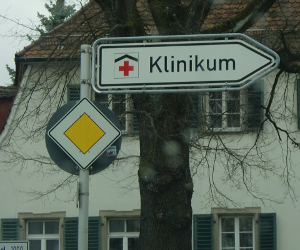
\includegraphics[width=0.3\textwidth]{plots/var_diff-klinikum_small.png} 
  }
  \subfigure[Test image 2]{
    \label{subfig:colorcheckerimg}
    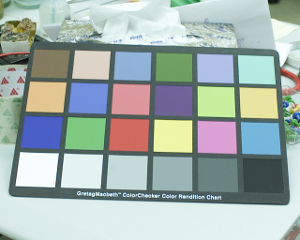
\includegraphics[width=0.3\textwidth]{plots/var_diff-colorchecker_small.png} 
  }
  \subfigure[Test image 3]{
    \label{subfig:stuffimg}
    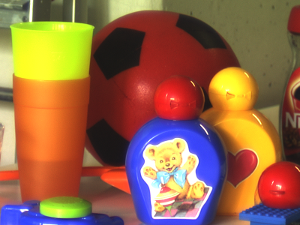
\includegraphics[width=0.3\textwidth]{plots/var_diff-stuff_small.png} 
  }
  \subfigure[$\beta$-map for \autoref{subfig:klinikumimg}]{
    \label{subfig:klinikum}
    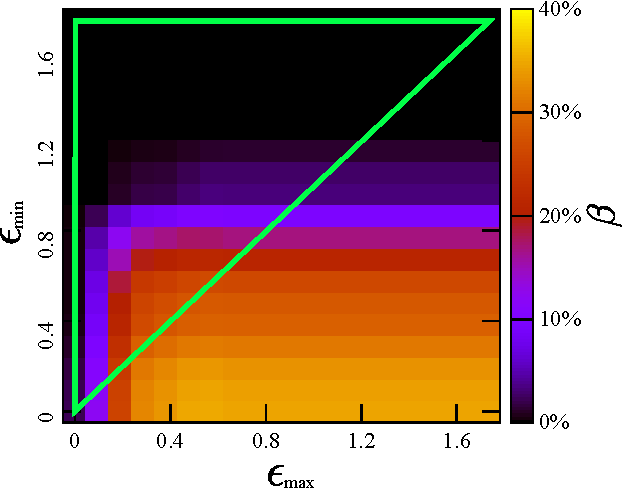
\includegraphics[width=0.31\textwidth]{plots/var_diff-klinikum.pdf} 
  }
  \subfigure[$\beta$-map for \autoref{subfig:colorcheckerimg}]{
    \label{subfig:colorchecker}
    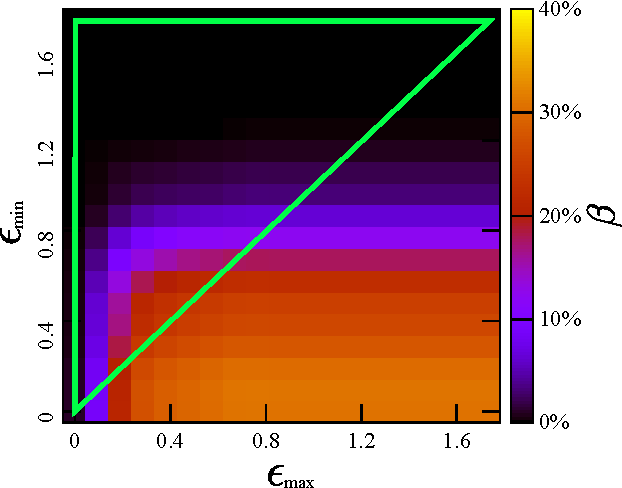
\includegraphics[width=0.31\textwidth]{plots/var_diff-colorchecker.pdf} 
  }
  \subfigure[$\beta$-map for \autoref{subfig:stuffimg}]{
    \label{subfig:stuff}
    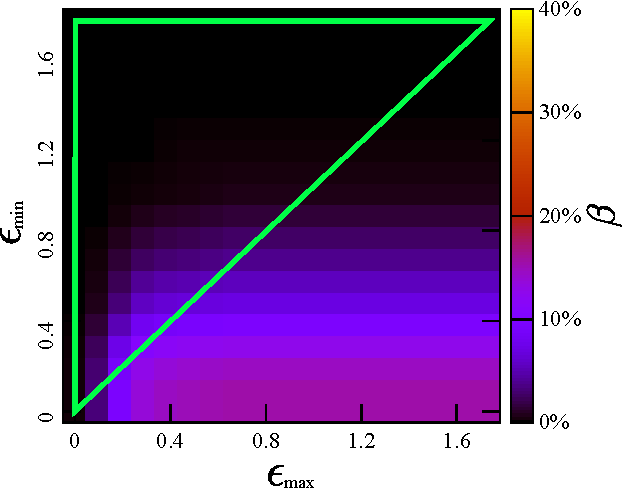
\includegraphics[width=0.31\textwidth]{plots/var_diff-stuff.pdf} 
  }
  \caption[Brute force determination of good values for $\epsilon_\text{min}$ and $\epsilon_\text{max}$]{Brute force determination of good values for $\epsilon_\text{min}$ and $\epsilon_\text{max}$. The first row contains the used images. The plot located below an image is its $\beta$-map, where brighter intensities (more yellow) represent higher color coverage. The green rectangle show the reasonable boundary for $\epsilon_\text{min}$ and $\epsilon_\text{max}$.}
  \label{fig:distanceparameterplots}
\end{figure}






\clearpage

\section{Tests with Synthetic Data}
\label{sec:syntheticdata}

\subsection{Experimental Setup}
\label{subsec:syntheticDataExperimentalSetting}

To examine the capabilities of the actual CRF estimation, a perfect observation set is assumed. The data acquisition step analyzed in the previous section is skipped and synthetic data is generated instead. A set of $N = 1500$ color triples ($C_1$, $C_2$, $C_{\text{edge}}$) is computed by picking the region colors $C_1$ and $C_2$ randomly for every color triple. Then, \autoref{eq:linearcombination} is used to get $C_{\text{edge}}$ with $\alpha = 0.5$. Now the situation is as in \autoref{subfig:irradiance}, an ideal CCD sensor is simulated. To emulate image intensity (\autoref{subfig:intensity}), a particular CRF $f$ is applied to all the colors in each color triple. In this chapter $f$ is a gamma curve with $\gamma \in \left\{0.2, 0.4, 0.6, 0.8, 1.0\right\}$. Note that ``more than $92 \%$ of the real-world digital camera CRFs in the DoRF database lie inbetween $r^{0.2}$ and $r^{0.6}$'' \cite{ng_cvpr07}. Hence, a linear gamma curve ($\gamma = 1.0$) is a quite unusual CRF.



\subsection{Error Measure}
\label{subsec:syntheticDataErrorMeasurement}

For the evaluation, an error function $\Psi(h_1, h_2)$ is introduced, which measures the dissimilarity of two distinct normalized two-dimensional functions $h_1$ and $h_2$.
\begin{equation}
	\Psi(h_1, h_2) = \frac{1}{M} \sum\limits_{i=1}^M \left( h_1\left(\frac{i}{M}\right) - h_2\left(\frac{i}{M}\right) \right)^2; \ \ M > 0 \enspace ,
	\label{eq:errfuncF1F2dissimilaritymeasure}
\end{equation}
where $M$ is the number of samples. For an illustration see \autoref{fig:errorfunctionPSI}. The left factor $1/M$ normalizes the error such that $\Psi \in \left[0;1\right]$, independent of $M$. The results in the following are obtained with $M = 1024$.
\begin{figure}[bt]
  \centering
  \subfigure[Example]{
    \label{subfig:exampleMeq6}
    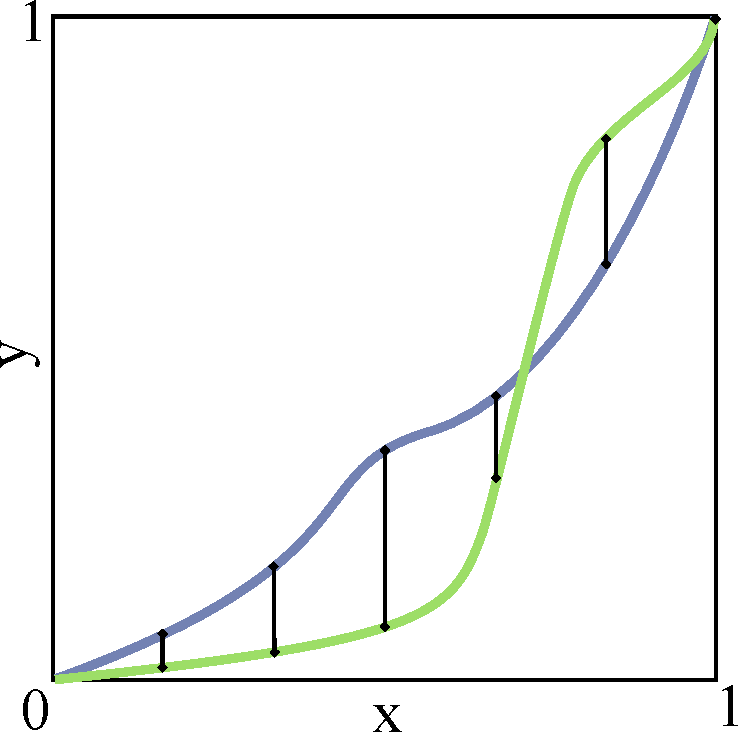
\includegraphics[width=0.3\textwidth]{images/error_function_psi_illustration.pdf} 
  }
  \subfigure[Example for maximum error]{
    \label{subfig:exampleMaxErr}
    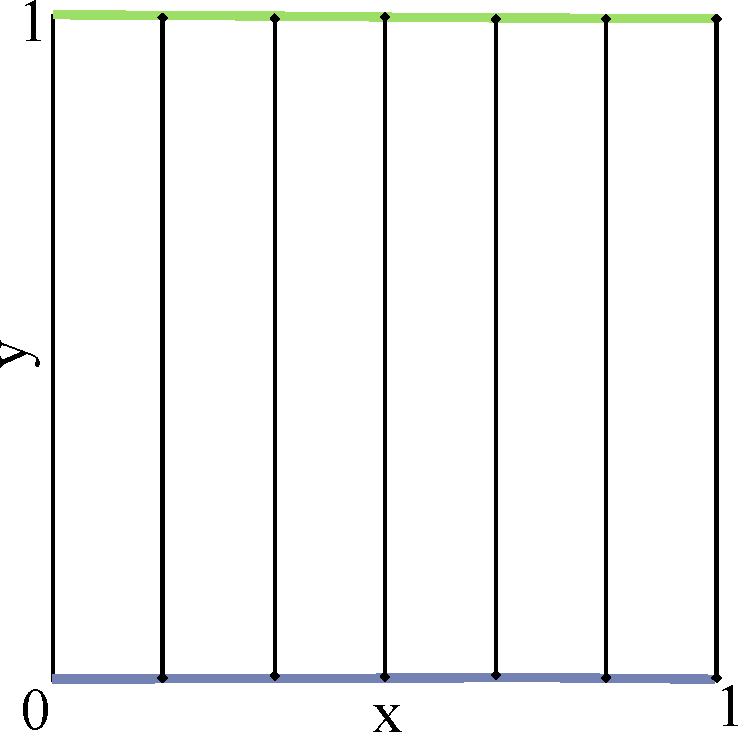
\includegraphics[width=0.3\textwidth]{images/error_function_psi_MAX_illustration.pdf} 
  }
  \caption[Error function illustration]{Error function illustration. $M$ is set to 6 for convenience. \autoref{subfig:exampleMeq6} shows two typical functions. The error is computed by adding up the length of the six black vertical lines squared each. The result is divided by $M$. An example which yields the maximum error function value is given in \autoref{subfig:exampleMaxErr} with $\Psi(h_1(x) = 0, h_2(x) = 1) = 1$.}
  \label{fig:errorfunctionPSI}
\end{figure}


\subsection{Results}
\label{subsec:syntheticDataResults}

In this section we will discuss the obtained results for four exemplary configurations of $(\kappa, \nu) \in \left\{ (3,3), (5,5), (5,7), (7,7) \right\}$. S. Lin, the author of \cite{Lin04radiometriccalibration}, proposed $\kappa = \nu = 5$, \hbox{i.e.} the number of kernels for the GMM $\kappa$ is set to 5, as well as the number of eigenvectors $\nu$ used for the PCA model.

The parameter $\lambda$ -- a weighting factor -- adjusts the impact of the \emph{prior model} based on the DoRF database versus the \emph{likelihood function}, which reflects the gathered data. For an explanation see \autoref{sec:radcal}. With increasingly large $\lambda$, more influence is passed to the information from the specific image (or from the image set). For very small $\lambda$, the estimated CRF is mainly based on the outcome of the EM algorithm, based on DoRF and controlled by $\kappa$ and $\nu$. 
\begin{figure}[tb]
	\centering
	\subfigure[$\kappa$ = 3; $\nu$ = 3]{
 	 \label{subfig:goodlambda3k3p}
 	 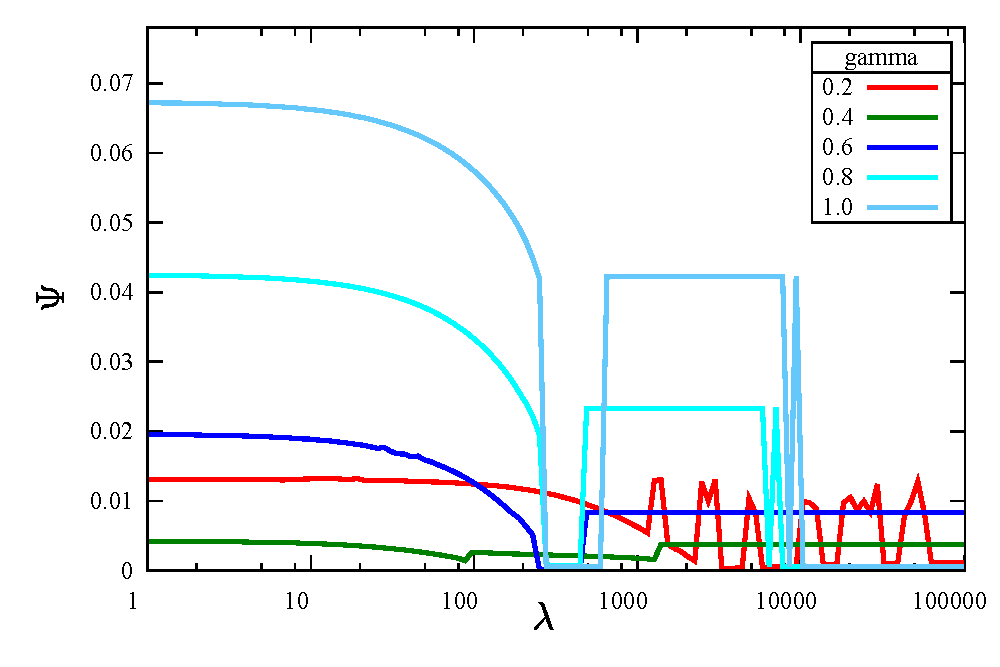
\includegraphics[width=0.483\textwidth]{plots/kernels3components3.pdf} 
  }
	\subfigure[$\kappa$ = 5; $\nu$ = 5]{
 	 \label{subfig:goodlambda5k5p}
 	 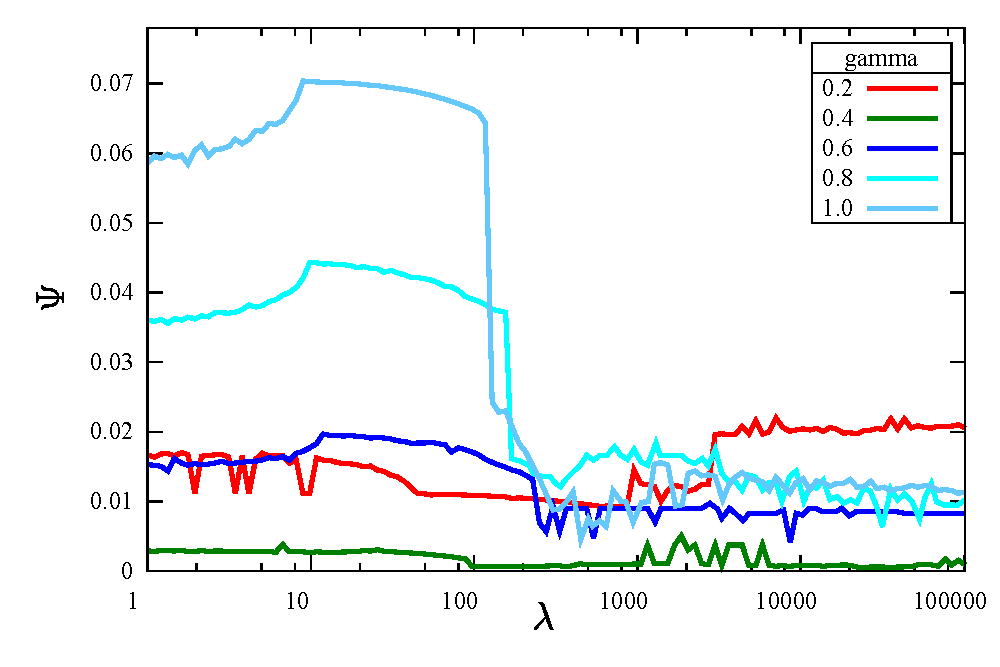
\includegraphics[width=0.483\textwidth]{plots/kernels5components5.pdf} 
  }
  \subfigure[$\kappa$ = 5; $\nu$ = 7]{
 	 \label{subfig:goodlambda5k7p}
 	 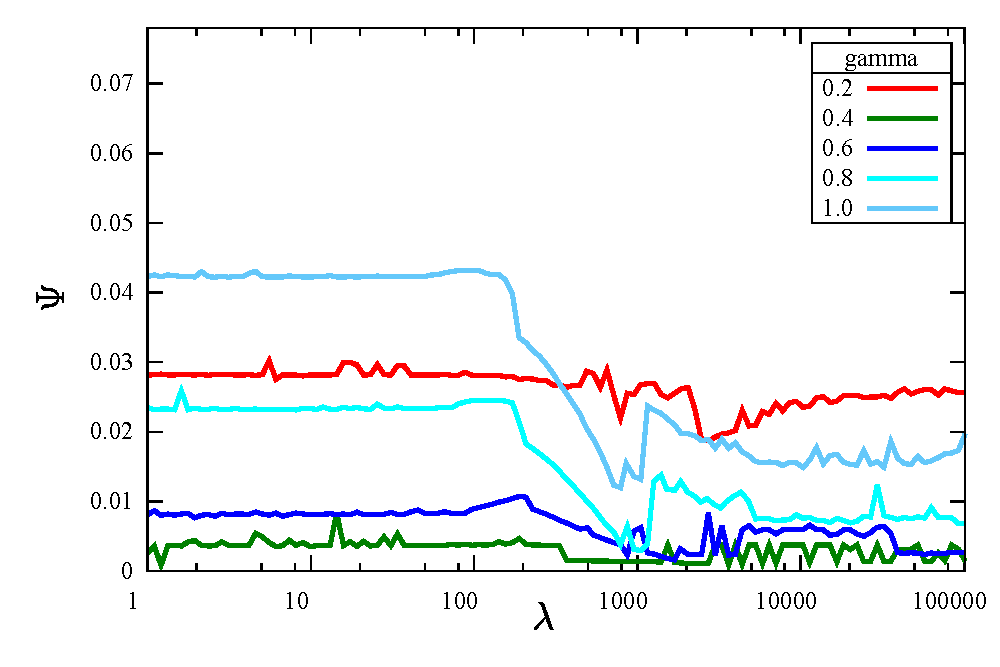
\includegraphics[width=0.483\textwidth]{plots/kernels5components7.pdf} 
  }
  \subfigure[$\kappa$ = 7; $\nu$ = 7]{
 	 \label{subfig:goodlambda7k7p}
 	 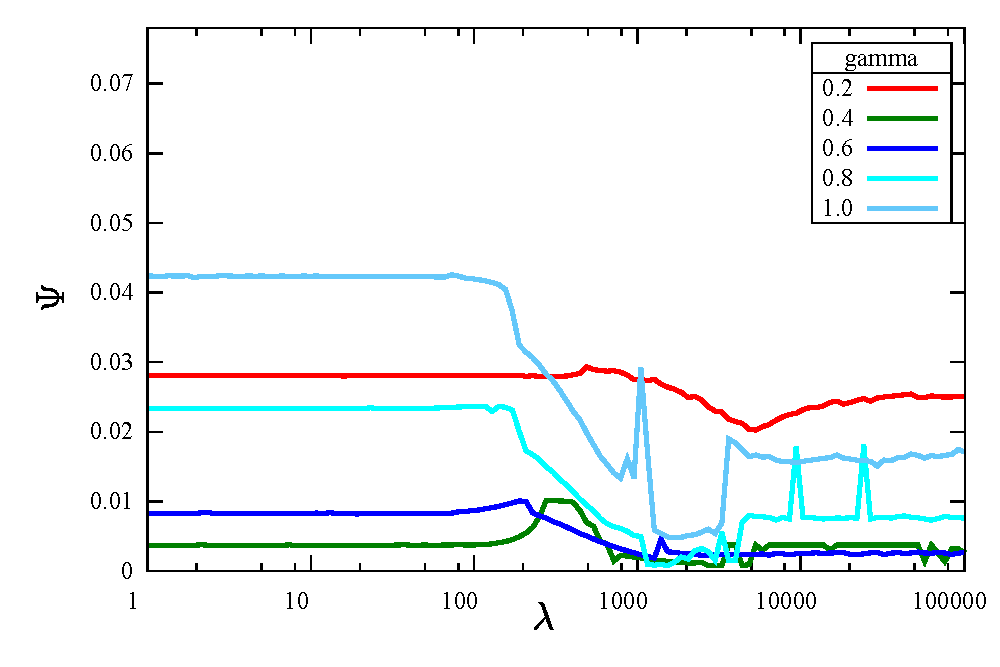
\includegraphics[width=0.483\textwidth]{plots/kernels7components7.pdf} 
  }
  \caption[Determination of balanced value for $\lambda$]{Determination of balanced value for $\lambda$. The error measurements $\Psi$ of the estimated curve to the ground-truth inverse CRF are visualized for four different configurations of $(\kappa, \nu)$ and five different gamma curves each. The presented curves interpolate between more than 120 logarithmic distributed measurements per gamma curve.}
	\label{fig:goodlambda}
\end{figure}

Considering perfect conditions as is the case with the above presented synthetic data, a very large value of $\lambda$ might be preferred. This means, that the examined image exhibits many distinct but uniform regions with almost no noise and thus the observation set is very well compiled, \hbox{e.g.} the color coverage factor $\beta$ reaches almost $100 \%$. 

Note that not even with $\lambda \rightarrow \infty$ the method is highly influenced by the ground-truth (\hbox{i.e.} $\Psi \rightarrow 0$) for many CRFs, because the optimization step -- starting from the DoRF mean curve $g_\text{DoRF}$ -- is still very much dependent on the PCA representation of the inverse CRF, which again is based on DoRF. So for this method, prior knowledge can not be \emph{switched off} and thus it is not a good choice if the examined images are taken by cameras with very unusual CRFs like a linear curve (in case of gamma curves: $\gamma = 1.0$).

Interpretation approaches for observations, which the results for all examined parameter setups have in common, are presented in the following on page \pageref{subsubsec:commonobservations}. This is continued by setup-specific observations. The actual results are shown in \autoref{fig:goodlambda}. Note the log scale on the horizontal axis ($\lambda$).



\clearpage

\subsubsection{Common Observations for all Settings}
\label{subsubsec:commonobservations}

For all parameter settings in \autoref{fig:goodlambda}, the (quite) linear CRFs ($\gamma = 1.0$ and $\gamma = 0.8$) have at least for $1 \leq \lambda \leq 200$ a very high error, \hbox{i.e.} the estimated function and the ground-truth are quite dissimilar. The reason is that they differ the most from $g_\text{DoRF}$. In contrast, the error measurements presented in green ($\gamma = 0.4$) consistently exhibit a very small error. Hence, $g_\text{DoRF}$ must be most similar to a gamma curve with $\gamma = 0.4$. Therefore, the measured values are mostly below $\Psi < 0.005$ for nearly any value of $\lambda$.

The trend of the red curve, representing the error measurements for a gamma curve with $\gamma = 0.2$, differs from the others. Except for the measurements in \autoref{subfig:goodlambda3k3p}, $\Psi$ does not get significantly smaller by increasing $\lambda$. In \autoref{subfig:goodlambda5k5p}, $\Psi$ even increases. Here, $\Psi$ for $\lambda = 10000$ is about $90\%$ larger than for $\lambda = 500$. Starting from a particular $\lambda$, even the quite unusual CRF, the linear curve ($\gamma = 1.0$), outperforms this gamma curve. We can not explain this phenomenon so far. 

For fixed $\nu$, but varying number of kernels for the Gaussian mixture model $\kappa$, an interesting observation can be extracted by comparing \autoref{subfig:goodlambda5k7p} to \autoref{subfig:goodlambda7k7p}. The two plots do not differ very much. Indeed, \autoref{subfig:goodlambda7k7p} looks like a smoothed version of \autoref{subfig:goodlambda5k7p}. Although the presumable expectation would be, that $\Psi$ varies more for a larger number of kernels than for smaller $\kappa$, the opposite is observed.



\subsubsection{Parameter-specific Observations}
\label{subsubsec:paramspecificobservations}

The error for small $\lambda$ is much larger for the settings presented in the first row than for those in the second row. We observed, that the number of used eigenvectors $\nu$ has significant impact on the shape of the estimated inverse CRF, what could be a reason for this effect.

In \autoref{subfig:goodlambda3k3p}, the trends of the blue curves ($\gamma \in \left\{0.8, 1.0\right\}$) exhibit significant unexpected changes. Around $\lambda \approx 800$, the previously decreasing or very low error measurements turn into horizontal lines until $\lambda \approx 10000$. A possible explanation for this effect is, that the LM minimization converges at a local minimum for several consecutive values of $\lambda$.

Regarding the curves with $\gamma \in \left\{0.6, 0.8, 1.0\right\}$ in \autoref{subfig:goodlambda5k5p}, another interesting aspect is the at first monotonically increasing error function values until $\lambda \approx 12$, where $\Psi$ suddenly decreases. A possible explanation for this effect is given by example. The prior model is a Gaussian mixture model with $\kappa$ kernels. A (inverse) CRF is represented by a $\nu$-dimensional vector. Without loss of generality, let $\nu = 2$ and $\kappa = 4$. So there is a two-dimensional space with four two-dimensional Gaussian bells. The ground-truth curve and the estimated curve are referred to as $\vec{p}_{\text{gt}}$ and $\vec{p}_{\text{est}}$. For a very small $\lambda = 1$, $\vec{p}_{\text{est}}$ is near the point representing the mean curve $\vec{p}_{\text{mean}}$. With increasing $\lambda$, the influence of the prior knowledge slowly decreases and thus $\vec{p}_{\text{est}}$ starts drifting towards the ground-truth $\vec{p}_{\text{gt}}$. But on the path from $\vec{p}_{\text{mean}}$ to $\vec{p}_{\text{gt}}$ some \emph{hurdles} (the Gaussian kernels) have to be passed, which -- if the influence of the prior model is still too high -- can \emph{pull} $\vec{p}_{\text{est}}$ into the wrong direction temporarily. But starting from a specific $\lambda \approx 12$, the \emph{pulling capabilities} of the kernels are not sufficient anymore and $\vec{p}_{\text{est}}$ continues traveling into the direction of its desired destination $\vec{p}_{\text{gt}}$. This process is outlined in \autoref{fig:lambdapath}. The image can be seen as an excerpt of the two-dimensional (inverse) CRF space using the PCA representation. Note that the distance between $\vec{p}_{\text{est}}$ and $\vec{p}_{\text{gt}}$ slightly increases for small $\lambda$ as pointed out above.

\begin{figure}[tb]
	\centering
		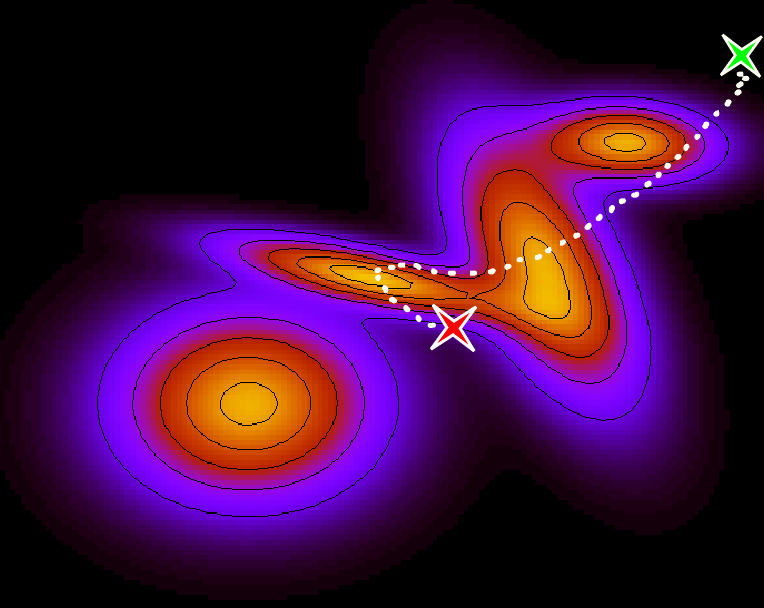
\includegraphics[width=0.5\textwidth]{images/lambda_path.png}
	\caption[Sketch of $\lambda$ influence]{Sketch of $\lambda$ influence. The red star depicts $\vec{p}_{\text{mean}}$ and the green star $\vec{p}_{\text{gt}}$. The dotted white line sketches the path of $\vec{p}_{\text{est}}$, when $\lambda$ is increasing. An exemplary GMM obtained by the EM algorithm is visualized by the underlying map.}
	\label{fig:lambdapath}
\end{figure}






\clearpage

\section{Stability Tests}
\label{sec:stability}

Purposely, neither the approach from \autoref{sec:capabilitiesofdataacqu} nor the one from \autoref{sec:syntheticdata} covered the whole algorithm as presented in \autoref{subsec:radcalalgo}. The two main steps, the observation set formation and the optimization step, were treated separately -- independently from each other -- to find reliable settings for the most significant parameters. Hence, the goal of this part of the thesis is to evaluate the method considering the \emph{entire} procedure, while using the previously obtained knowledge on the crucial parameters. 


\subsection{Prerequisites}
\label{subsec:stabilityPrerequisites}

A commonly used approach is to assess the robustness of a method. Therefore 8 sets of images from 8 different cameras were compiled with an average of about 50 images per camera. Only images with a very high probability not being post-processed in image manipulation tools like ``Adobe Photoshop'' \cite{photoshop} or ``GIMP, The GNU Image Manipulation Program'' \cite{gimp} were taken into the sets. The reason is that such software can manipulate images in a way, that an estimation of the actually applied CRF gets impossible. Therefore the collected photos were either
\begin{itemize}
	\item photographs from our own cameras, which are certainly in their original state or
	\item amateur shots from online resources like \emph{picasaweb}\footnote{\url{http://picasaweb.google.com/}} or \emph{flickr}\footnote{\url{http://www.flickr.com/}} tagged ``not manipulated'' or similarly.
\end{itemize}
Many prestigious camera manufacturers are covered: Canon, Sony, Casio, FujiFilm and two camera models each from Kodak and Nikon. Both professional camera models like the Canon EOS 400D Rebel XTi and cheaper models for beginners like the Casio Exilim EX-S600 are examined. 

We also included about 250 samples from a publicly available database of RGB color images \cite{ciurea2003large} in our tests. It consists of 11000 images and is primarily intended for color constancy research. The assumption is, that for each image in the database, the CRF is approximately similar. Hence, we can test the robustness of the examined method for this set of images, too. This database is referred to as ``Funt database'' in the following. Due to the fact, that the images in this database are relatively small sized ($360 \times 240$ pixels), the size of the patches was decreased to $W = H = 12$ and thus also the maximum dilation distance is set to $2$.



\subsection{Leave-One-Out Approach}
\label{subsec:stabilityLOO}

As the name suggests, the leave-one-out (LOO) technique uses only a single observation -- in this case only one estimated inverse CRF from a whole set of inverse CRFs -- per iteration to obtain error measurements. The successive steps for this evaluation approach are described in the following, while a simplified visualization of the functional principle is presented in \autoref{fig:leaveOneOut}.

\begin{figure}[tb]
	\centering
	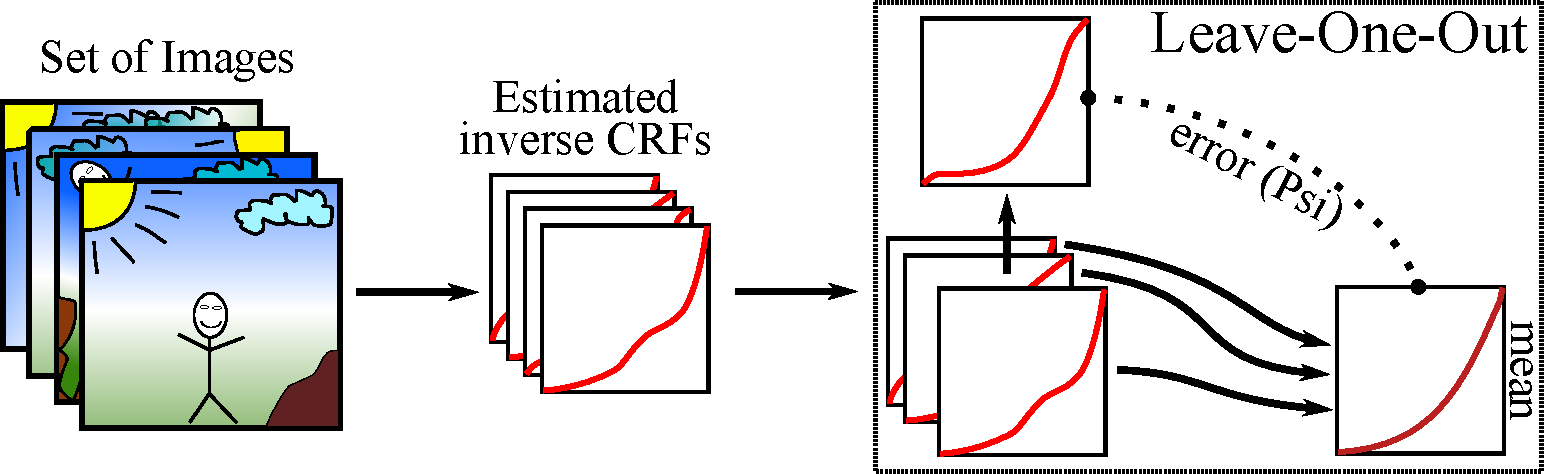
\includegraphics[width=0.8\textwidth]{images/loo_description.pdf}
	\caption[Leave-one-out overview]{Leave-one-out overview. This figure represents a simplified version, where only one channel is shown. Note that the error is measured between the \emph{left out} curve and the mean curve computed over the \emph{other} curves.}
	\label{fig:leaveOneOut}	
\end{figure}

Given a set of $n$ images taken with the same camera, the algorithm as presented in \autoref{subsec:radcalalgo} is conducted on each image seperately. This produces a set $\mathcal{G}$ of $n$ inverse CRF triples 
\begin{equation}
	\mathcal{G} = \left\{\vec{g}_i = 
	\begin{pmatrix} g_{i_\text{red}} \\ g_{i_\text{green}} \\ g_{i_\text{blue}} \end{pmatrix}; \ i=1 \ldots n\right\} \enspace ,
	\label{eq:setOfInverseCRFs}
\end{equation}
where for each image three inverse CRFs -- one for each channel (red, green and blue) -- are estimated, \hbox{i.e.} altogether $3n$ inverse camera response function.

Now a set $\mathcal{E}$ of three-dimensional error vectors $\vec{e}_i \in \mathcal{E}$ is obtained by evaluating
\begin{equation}
	\vec{e}_i = 
	\begin{pmatrix}
		e_{i_\text{red}}   &=& \Psi \left( g_{i_\text{red}}, \mathrm{mean} \left( \mathcal{G}_\text{red} \setminus \left\{ g_{i_\text{red}} \right\} \right) \right) \\
		e_{i_\text{green}} &=& \Psi \left( g_{i_\text{green}}, \mathrm{mean} \left( \mathcal{G}_\text{green} \setminus \left\{ g_{i_\text{green}} \right\} \right) \right) \\
		e_{i_\text{blue}}  &=& \Psi \left( g_{i_\text{blue}}, \mathrm{mean} \left( \mathcal{G}_\text{blue} \setminus \left\{ g_{i_\text{blue}} \right\} \right) \right)
	\end{pmatrix}
	\label{eq:errorVector}
\end{equation}
for each $\vec{g}_i \in \mathcal{G}$. $\mathcal{G}_c$ is the set of inverse CRFs for a particular channel $c \in \{\text{red}, \text{green}, \text{blue}\}$ extracted from $\mathcal{G}$. $\Psi$ is the error measurement from \autoref{eq:errfuncF1F2dissimilaritymeasure} and the function $\mathrm{mean}$ computes the mean curve of the given set of inverse CRFs. The best and worst case for each channel, \hbox{i.e.} the minimum error $e_\text{min}$ and maximum error $e_\text{max}$ are stored.

In the next step the mean error $\mu_c$ per channel $c$ is computed by 
\begin{equation}
	\mu_c = \frac{1}{n} \sum\limits_{i=1}^{n} e_{i_c} \enspace .
	\label{eq:meanErrorComputationPerChannel}
\end{equation}

Besides the mean error $\mu$, its standard deviation $\sigma$ is also a meaningful measurement. Therefore, $\sigma_c$ is obtained for each channel $c$ by
\begin{equation}
	\sigma_c = \sqrt{\sigma_c^2} = \sqrt{ \frac{1}{n} \sum\limits_{i=1}^{n} \left( e_{i_c} - \mu_c \right)^2 } \enspace .
	\label{eq:stddev}
\end{equation}

To get an overall measurement, \hbox{i.e.} for the entire camera and thus for all three channels combined, the joint mean error $\mu_\text{joint}$ and the joint standard deviation $\sigma_\text{joint}$ for all channels is computed as well.
\begin{eqnarray}
	\mu_\text{joint}    &=& \frac{1}{3 n} \sum\limits_{i=1}^{n} \left( e_{i_\text{red}} + e_{i_\text{green}} + e_{i_\text{blue}} \right) \enspace \text{and} \\
	\label{eq:meanErrorJoint}
	\sigma_\text{joint} &=& \sqrt{ \frac{1}{3 n} \sum\limits_{i=1}^{n} \left( \left( e_{i_\text{red}} - \mu_\text{joint} \right)^2 + \left( e_{i_\text{green}} - \mu_\text{joint} \right)^2 + \left( e_{i_\text{blue}} - \mu_\text{joint} \right)^2 \right) } \enspace .
	\label{eq:StdDevJoint}
\end{eqnarray}


\clearpage

\subsection{Results}
\label{subsec:stabilityResults}

Our results presented in this section were obtained using different parameter setups for $\kappa$, $\nu$ and $\lambda$. The main quality factor is the joint mean error $\mu_\text{joint}$, \hbox{i.e.} the smaller $\mu_\text{joint}$ is, the more robust is the method for a particular set of images. For these tests, images with a color coverage factor $\beta < 5\%$ were ignored. 

The examination of the parameter $\lambda$ in \autoref{sec:syntheticdata} leads to the assumption, that the robustness for small $\lambda$ is better than for big $\lambda$. The reason is the merely minor impact of the image-specific information for small $\lambda$. Hence, the estimation is mainly affected by the prior model, which is equal for every image. Consequently, the resulting inverse CRFs will not differ a lot and thus $\mu_\text{joint}$ will be significantly lower than for large $\lambda$. Note that a small $\mu_\text{joint}$ does not necessarily implicate good estimates in comparison to the unknown ground-truth inverse CRF.

\autoref{fig:lambdavariation} illustrates the increasing value for $\mu_\text{joint}$ for increasing $\lambda$. The two cameras Canon EOS 400D and Sony CyberShot DSC-W300 are compared directly. For all three presented configurations of $(\kappa, \nu) \in \left\{(3,3), (5,5), (7,7)\right\}$, the inequation $\mu_\text{joint}(100) < \mu_\text{joint}(1000) < \mu_\text{joint}(10000)$ holds. The only exception is for the Funt database. There, for the settings $(\kappa,\nu) \in \left\{ (3,3), (5,5) \right\}$, $\mu_\text{joint}(10000) < \mu_\text{joint}(1000)$.
\begin{figure}[btp]
  \centering
	 \subfigure[Canon EOS 400D -- $\kappa$ = 3; $\nu$ = 3]{
 	 \label{subfig:canoneos3k3c_lambda_diff}
 	 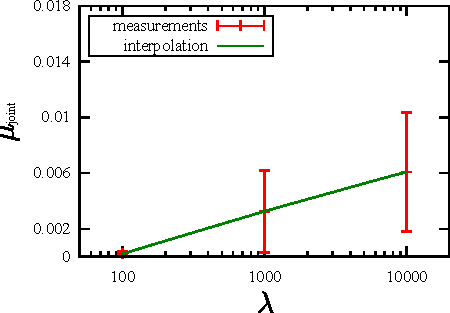
\includegraphics[width=0.4\textwidth]{plots/canoneos3k3c_lambda_diff.pdf}
  }
  \subfigure[Sony CyberShot DSC-W300 -- $\kappa$ = 3; $\nu$ = 3]{
    \label{subfig:sony3k3c_lambda_diff}
    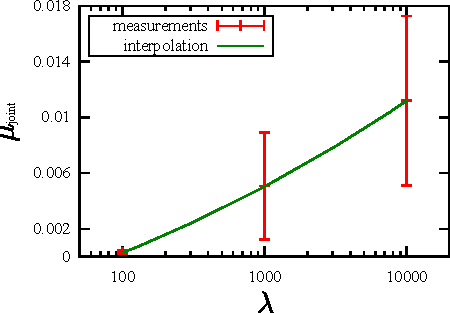
\includegraphics[width=0.4\textwidth]{plots/sony3k3c_lambda_diff.pdf}
  }
  \subfigure[Canon EOS 400D -- $\kappa$ = 5; $\nu$ = 5]{
 	 \label{subfig:canoneos5k5c_lambda_diff}
 	 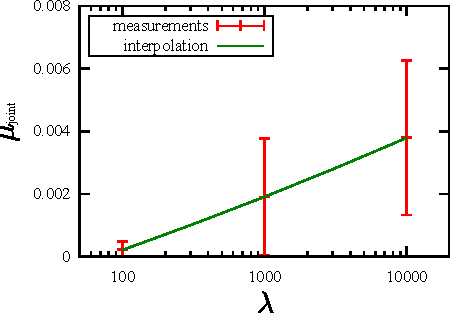
\includegraphics[width=0.4\textwidth]{plots/canoneos5k5c_lambda_diff.pdf}
  }
  \subfigure[Sony CyberShot DSC-W300 -- $\kappa$ = 5; $\nu$ = 5]{
    \label{subfig:sony5k5c_lambda_diff}
    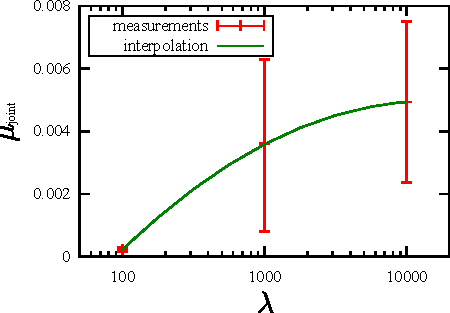
\includegraphics[width=0.4\textwidth]{plots/sony5k5c_lambda_diff.pdf}
  }
  \subfigure[Canon EOS 400D -- $\kappa$ = 7; $\nu$ = 7]{
 	 \label{subfig:canoneos7k7c_lambda_diff}
 	 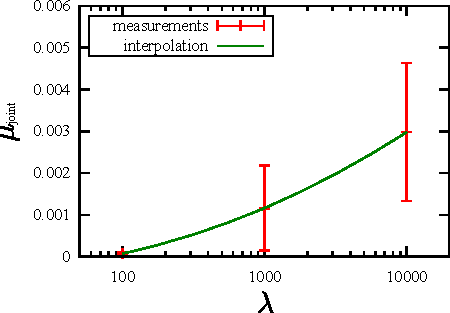
\includegraphics[width=0.4\textwidth]{plots/canoneos7k7c_lambda_diff.pdf}
  }
  \subfigure[Sony CyberShot DSC-W300 -- $\kappa$ = 7; $\nu$ = 7]{
    \label{subfig:sony7k7c_lambda_diff}
    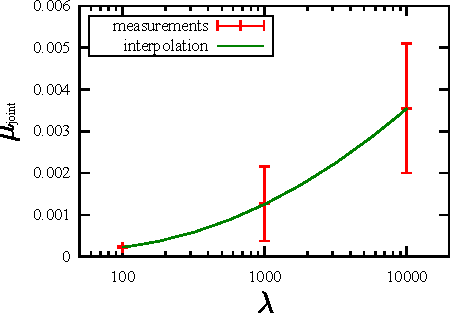
\includegraphics[width=0.4\textwidth]{plots/sony7k7c_lambda_diff.pdf}
  }
  \caption[Increasing $\mu_\text{joint}$ for increasing $\lambda$]{Increasing $\mu_\text{joint}$ for increasing $\lambda$. The red bars show the actual measurements and their standard deviations $\sigma_\text{joint}$. The green curve interpolates between the measurements. In each row, $\kappa$ and $\nu$ are fixed. Note the log scale on the horizontal axis.}
  \label{fig:lambdavariation}
\end{figure}

The overall best result in terms of robustness is presented in \autoref{tab:Canon EOS 400D Rebel XTi77100 - inText}. The first three columns represent the red, green and blue channel. In the last two rows of the fourth column, the two measurements from \autoref{eq:meanErrorJoint} are located. The most meaningful measurement $\mu_\text{joint}$ is printed in bold. Note the relatively small value of $\lambda = 100$. It is actually the smallest one used for this evaluation approach. Hence, the previously made assumption on $\lambda$ turned out to be true for our experiments. 

The worst observation, \hbox{i.e.} the largest value for $\mu_\text{joint}$, was observed for the highest used value of $\lambda = 10000$. It is presented in \autoref{tab:Kodak DX75903310000 - inText}. The mean joint error is about 200 times larger in comparison to the best case.
\begin{table}[tb]
  \centering
    \begin{tabular}{|c||c|c|c|c|}\hline
		   & \textbf{Red} & \textbf{Green} & \textbf{Blue} & \textbf{$\sum$} \\\hline\hline
      $e_\text{min}$ & 0.000053 & 0.000053 & 0.000053 &   \\\hline
      $e_\text{max}$ & 0.000363 & 0.000512 & 0.000605 &   \\\hline
      $\mu$          & 0.000079 & 0.000076 & 0.000087 & \textbf{0.000081} \\\hline
      $\sigma$       & 0.000019 & 0.000018 & 0.000029 & 0.000022 \\\hline
    \end{tabular}
  \caption{Best stability: Canon EOS 400D -- $\kappa$ = 7; $\nu$ = 7; $\lambda$ = 100}
  \label{tab:Canon EOS 400D Rebel XTi77100 - inText}
\end{table}
\begin{table}
  \centering
    \begin{tabular}{|c||c|c|c|c|}\hline
		   & \textbf{Red} & \textbf{Green} & \textbf{Blue} & \textbf{$\sum$} \\\hline\hline
      $e_\text{min}$ & 0.004425 & 0.002074 & 0.002261 &   \\\hline
      $e_\text{max}$ & 0.158236 & 0.085810 & 0.064222 &   \\\hline
      $\mu$          & 0.017749 & 0.015236 & 0.015869 & \textbf{0.016285} \\\hline
      $\sigma$       & 0.017430 & 0.013811 & 0.013130 & 0.014790 \\\hline
    \end{tabular}
  \caption{Worst stability: Kodak DX7590 -- $\kappa$ = 3; $\nu$ = 3; $\lambda$ = 10000}
  \label{tab:Kodak DX75903310000 - inText}
\end{table}

Some of the actually estimated inverse CRFs for the best and worst results as well as for an average case and some examples of the Funt database are presented in \autoref{fig:samplecurvesStability}. The effects of having good or bad robustness, \hbox{i.e.} small or large values of $\mu_\text{joint}$, can obviously be observed in these plots. In \autoref{fig:meancurvesred}, the \emph{mean} inverse CRFs for the best and the worst result are shown. They are both very similar to the DoRF mean curve.

\begin{figure}[bt]
  \centering
  \subfigure[Canon EOS 400D -- $\kappa$ = 7; $\nu$ = 7; $\lambda$ = 100]{
 	 \label{subfig:bestSampleCurves}
 	 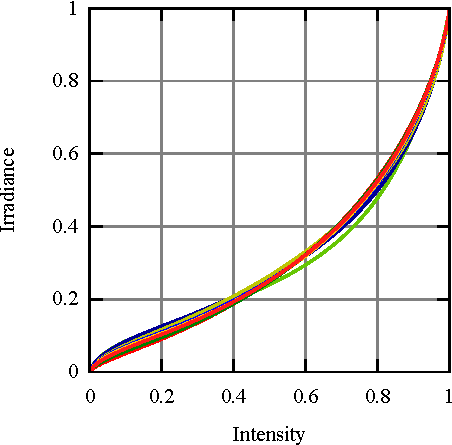
\includegraphics[width=0.4\textwidth]{plots/best_sample_curves.pdf}
  }
  \subfigure[Kodak DX7590 -- $\kappa$ = 3; $\nu$ = 3; $\lambda$ = 10000]{
 	 \label{subfig:worstSampleCurves}
 	 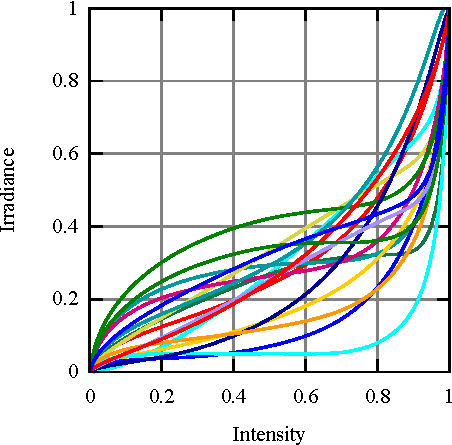
\includegraphics[width=0.4\textwidth]{plots/worst_sample_curves.pdf}
  }
  \subfigure[Nikon D40 -- $\kappa$ = 5; $\nu$ = 5; $\lambda$ = 10000]{
 	 \label{subfig:avgSampleCurves}
 	 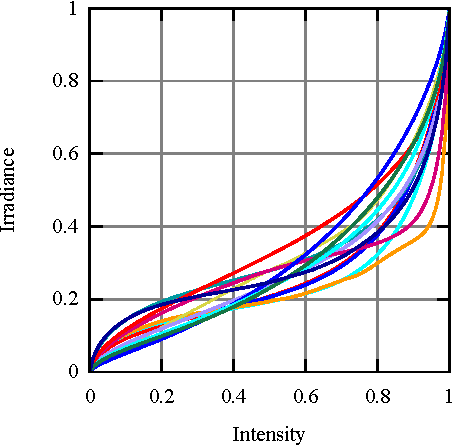
\includegraphics[width=0.4\textwidth]{plots/average_sample_curves.pdf}
  }
  \subfigure[Funt database -- $\kappa$ = 7; $\nu$ = 7; $\lambda$ = 10000]{
 	 \label{subfig:funtSampleCurves}
 	 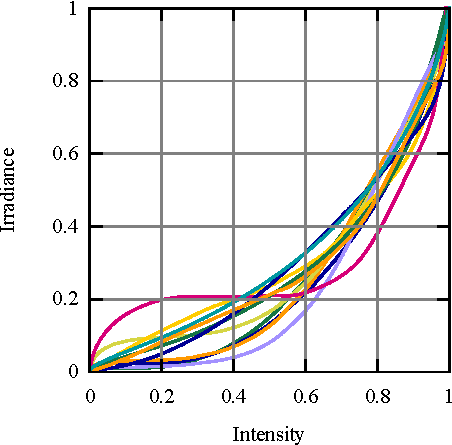
\includegraphics[width=0.4\textwidth]{plots/funt_sample_curves.pdf}
  }
  \caption[Sample inverse CRF estimates (stability test)]{Sample inverse CRF estimates for the best (\autoref{subfig:bestSampleCurves}) and the worst (\autoref{subfig:worstSampleCurves}) stability. Samples for an average value of $\mu_\text{joint}$ are presented in \autoref{subfig:avgSampleCurves} and representative estimates from the Funt database in \autoref{subfig:funtSampleCurves}.}
  \label{fig:samplecurvesStability}
\end{figure}

\begin{figure}[bt]
	\centering
 	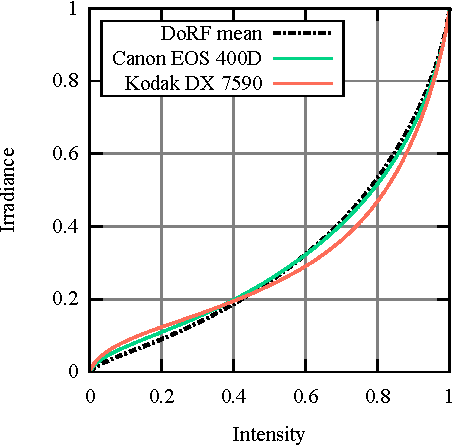
\includegraphics[width=0.35\textwidth]{plots/best_vs_worst_mean_red_channel.pdf}
	\caption[Best and worst mean curve]{Mean curves for best (green) and worst (red) stability (for the red channel). The dotted curve represents the mean inverse CRF from DoRF.}
\label{fig:meancurvesred}	
\end{figure}

To get an overall impression of the obtained results, we created a plot of all tested datasets and parameters (see \autoref{fig:bigcomparison}). It reflects the previously made conclusions. Note that the figure is subdivided into three distinct plots, one for each configuration of $(\kappa, \nu)$, illustrated by the dashed vertical lines. The horizontal axis differentiates the values of $\lambda$ and the vertical axis shows the error measure $\mu_\text{joint}$. The most stable results, independently of the chosen parameters, are obtained for the set of images from Canon EOS 400D and from the Funt database. Some sample estimated inverse CRFs from the Funt database are shown in \autoref{subfig:funtSampleCurves}. 

It turned out, that if only small values for $\kappa$ and $\nu$ are chosen, \hbox{e.g.} $(3,3)$, worse stability is measured than for larger values. Furthermore, the best results in terms of both, stability and similarity to the ground-truth curve combined, are the results with the smallest values of $\mu_\text{joint}$ for the largest value of $\lambda = 10000$. The reason is, that even though the prior model has only little impact on the estimates, the algorithm returns quite similar inverse CRFs. Hence, the image-specific observation set seems to be rather well compiled and also the CRF estimation step produced good results. All in all, the entire algorithm reached rather good performance.

Some additional tables for two different parameter setups are presented in \autoref{chap:additionalTables}.

\begin{figure}[bt]
	\centering
 	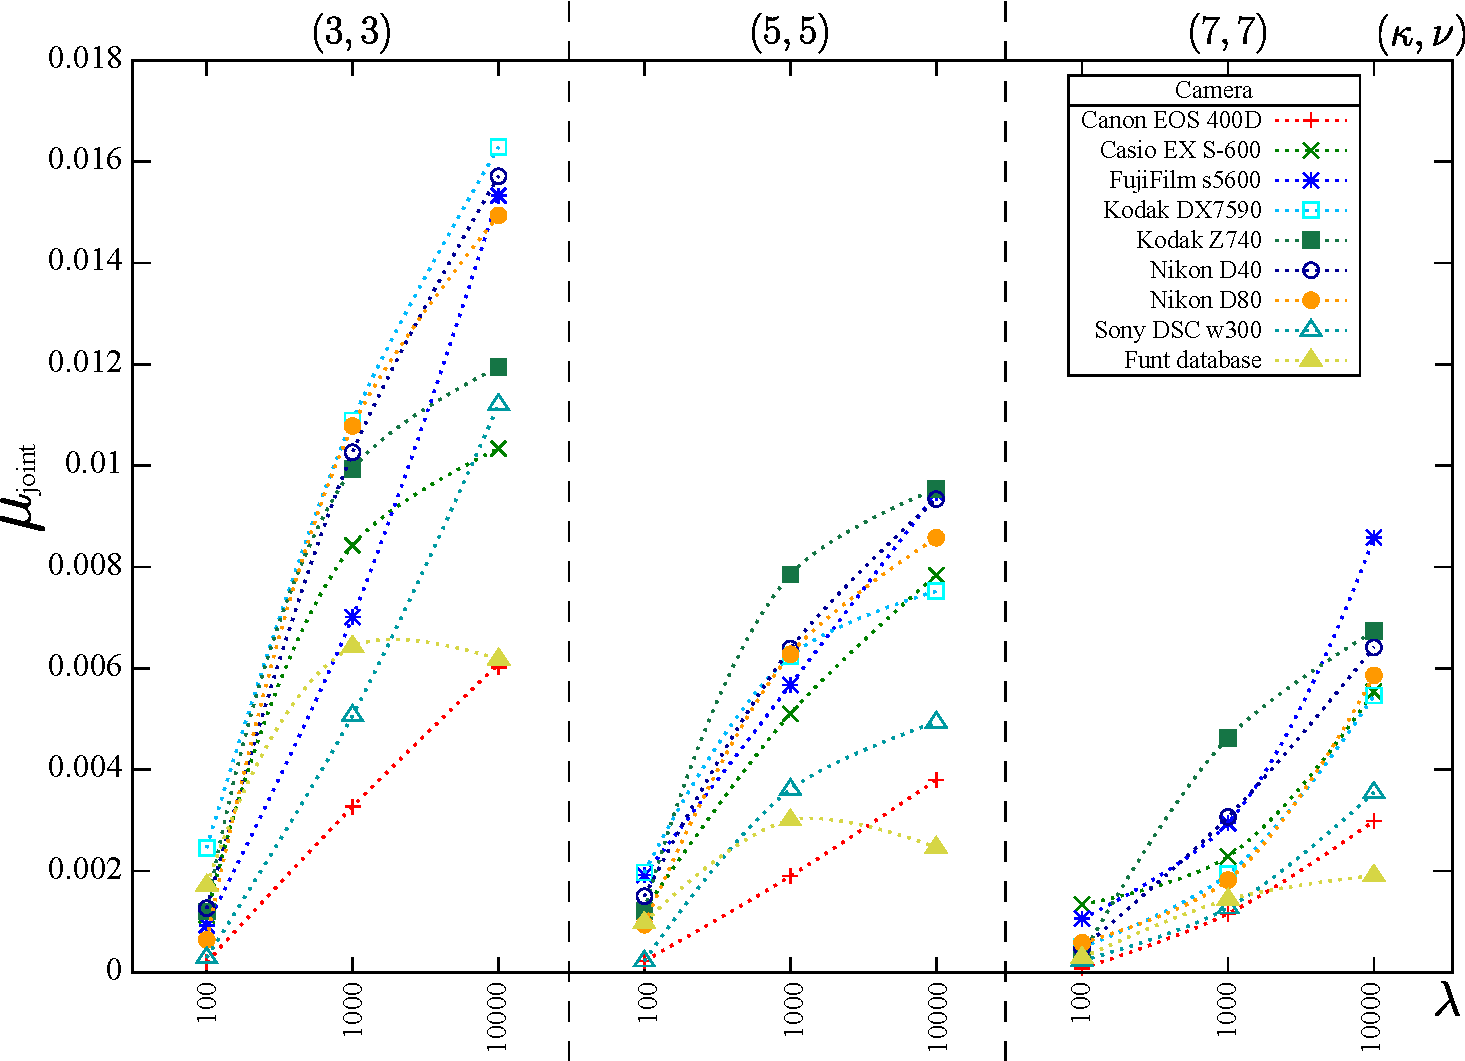
\includegraphics[width=0.95\textwidth]{stabilitytest/big_comparison.pdf}
	\caption[Overview of all obtained results]{Overview of all obtained results. The dotted curves connect the consecutive measurements of the same camera.}
\label{fig:bigcomparison}	
\end{figure}